\section{Read-Eval-Print Loops}
\label{sec:repl}

Many programming languages come with an interactive environment. This
interactive environment is an interface to the programming language's execution
engine. One common form of such an environment is an interface in which
expressions in a programming language are typed by the user, after which the
results of that expression are printed back to the user. Such an environment is
called a Read-Eval-Print Loop (REPL), although many different names are known,
including but not limited to \emph{language shell}, \emph{command-line
  interpreter} or \emph{interactive interpreter}. In this report the term REPL
is chosen, because it conveys the notion of such an interactive environment
well.

\subsection{Origin of REPLs}
\label{ssec:repl-origin}

The Lisp programming language is one of the first programming languages offering
such an interactive environment~\cite{Noyes92}. The name REPL comes from the
Lisp functions that implement it:

\begin{enumerate}
  \item The \texttt{read} function takes a user's input, which often is just one
    or several expressions as opposed to a complete compilation unit. It then
    parses this input and creates an AST.
  \item The AST created in the previous step is then passed on to the
    \texttt{eval} function, which evaluates it.
  \item The result yielded by the previous function is then printed out to the
    user by the \texttt{print} function.
  \item After having printed the result, the environment needs to \texttt{loop}
    back to the read state.
\end{enumerate}

Assuming the individual functions listed previously exist, a REPL can be created
in a single line of code simply by combining the functions:

\begin{lstlisting}[language=lisp]
(loop (print (eval (read))))
\end{lstlisting}

Lisp has a property called ``homoiconicity'': Lisp's syntax is similar to
its internal representation, resulting in the ability to infer a program's or
data object's state simply by reading its textual representation. Syntax and AST
are thus isomorphic, allowing data and code to be accessed and transformed
interchangeably.

In Lisp REPLs, therefore, arbitrary data objects yielded from a previous
expression can be used directly as input to the next expression. In programming
languages that do not belong to the Lisp family, homoiconicity is an unusual
feature. Interactive environments for these languages therefore often require
additional steps to read and evaluate expressions. This is part of the semantic
differences between the different names as mentioned in the introduction

\subsection{Advantages of REPLs}
\label{ssec:repl-advantages}

REPLs provide the ability to program interactively. Programming interactively
has multiple advantages.

When creating software solutions for an as of yet not well understood domain, it
is often not clear which data structures and algorithms are required. In such
cases, interactively developing and debugging software is an advantage over the
(oftentimes much slower) edit-compile-run-debug development style. This kind of
programming is called exploratory programming~\cite{Fritzson86}. Related to this
kind of exploration, programming interactively also provides a means for rapid
prototyping and bottom up programming~\cite{Graham93}.

The explorative and interactive features of a REPL also make it an excellent
tool for programmers to learn a new programming language. REPLs are also
combined with what is called literate programming to offer notebooks or language
playgrounds, as discussed in \cref{sec:literate-programming}.

\subsection{Execution model}
\label{ssec:execution-model}

Every programming language defines an execution model, which specifies how
programs written in that language are executed. Among others, it specifies what
an indivisible unit of work is (a \emph{compilation unit}) and in what order
these units are executed. The implementation of an execution model is a compiler
and/or an interpreter. The execution model of a REPL as shown in
\cref{fig:execution-model-repl} has a couple of differences with respect to that
of an interpreter or compiler.

One difference is what is considered an indivisible unit of work: a REPL might
accept singular expressions that a regular interpreter or compiler might
not. Usually the program is executed as a whole, without the need for smaller
blocks of execution. In contrast, when using a REPL, it might be desirable to be
able to execute only a single statement as one unit of execution. The AST output
of the parsing step, as shown in \cref{fig:execution-model-repl}, can therefore
be a smaller unit than an AST found in the ordinary execution model.

Another difference between a compiler or an interpreter and a REPL is that a
REPL needs to dynamically maintain an environment such that each new expression
can be analyzed and evaluated within the environment of previously executed
expressions. For every expression entered, it thus needs to apply the outlined
steps again and update the environment it maintains in memory with the new
results. This could result in a different order of evaluation than when for
example an interpreter executes a program as a whole.

\begin{figure}[t]
  \centering
  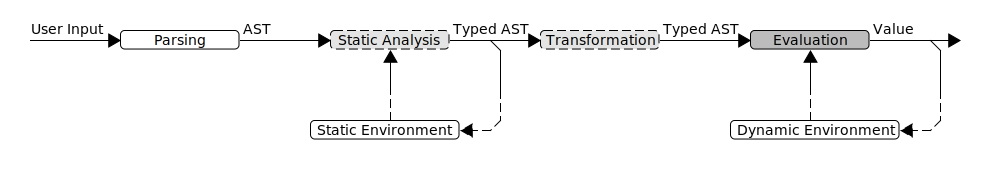
\includegraphics[width=\textwidth]{execution-model-repl}
  \caption{The execution model as shown in \cref{fig:spoofax-relations}, adapted
    for a REPL. The analysis and evaluation is done within the incrementally
    built environment of previously executed expressions.}
  \label{fig:execution-model-repl}
\end{figure}

\subsection{Functionality}
\label{ssec:repl-functionality}

Every REPL provided with a programming language has its own set of
functionality. However, a core set of functionalities, shared between all REPL
implementations, can be identified. To reach this core set of features,
well-known REPLs have been investigated and their features have been compiled
into a matrix as seen in \cref{table:feature-matrix}. These features are shortly
discussed below.

\begin{table}[]
\centering
\begin{tabular}{lccccccccc}
                                  & \rot{Python} & \rot{R} & \rot{\shortstack[c]{Common\\Lisp}} & \rot{\shortstack[c]{Haskell\\(GHCi)}} & \rot{Swift} \\
\toprule
Execution in context              & \cmark       & \cmark  & \cmark                             & \cmark                                & \cmark      \\
Input history                     & \cmark       & \cmark  & \cmark                             & \cmark                                & \cmark      \\
Automatic binding of previously yielded values & \xmark & \xmark & N/A                          & \xmark                                & \cmark      \\
Persistent input history          & \cmark       & \cmark  & \xmark                             & \cmark                                & \cmark      \\
Multiline input editing           & \cmark       & \cmark  & \cmark                             & \cmark                                & \cmark      \\
Redefining identifiers            & \cmark       & \cmark  & N/A                                & \cmark                                & \cmark      \\
Error reporting                   & \cmark       & \cmark  & \cmark                             & \cmark                                & \cmark      \\
Semantic code completion          & \cmark       & \xmark  & N/A                                & \xmark                                & \cmark      \\
Help or documentation system      & \cmark       & \cmark  & \cmark                             & \xmark                                & \xmark      \\
Additional commands to the REPL   & \xmark       & \xmark  & \cmark                             & \cmark                                & \cmark      \\
Nested REPLs to enable debugging  & \xmark       & \xmark  & \cmark                             & \xmark                                & \xmark      \\
\bottomrule
\end{tabular}
\caption{A feature comparison of several well-known REPLs}
\label{table:feature-matrix}
\end{table}

\paragraph{Execution in context} Expressions that are entered are executed
within the context of previous executions.

\paragraph{Input history} REPLs keep a history of inputs, such that previously
entered expressions can be retrieved.

\paragraph{Automatic binding of previously yielded values} When an expression
has been evaluated, the yielded result is bound to an automatically created
identifier, such that it can be reused easily in future expressions.

\paragraph{Persistent history} The input history as discussed previously can be
recorded into a file (either per-project or globally) to enable a persistent
history of input.

\paragraph{Multiline input editing} Some constructs in a programming language
naturally span multiple lines. REPLs therefore provide multiline input editors
that recognize incomplete code and promptly switch to a multiline environment
when required.

\paragraph{Redefining identifiers} When using a REPL in an exploratory manner,
it is not uncommon to want to redefine an identifier's type or to completely
reimplement a method. In this way, a REPL can be different than its host
language, especially if the host language is a functional language that does not
allow variables' values to change once initiated.

\paragraph{Error reporting} A REPL typically has the same error reporting
functionality as an interpreter or a compiler, meaning it prints the error
message accompanied by the corresponding section of the source code.

\paragraph{Semantic code completion} Semantic code completion is a helpful tool
to provide an overview of the often many APIs a developer works with, adding to
the explorative nature of a REPL. Note that this is a restriction of syntactic
completion, which is offered by all the studied REPLs.

\paragraph{Help or documentation system} The exploratory nature of a REPL means
that one will often see new methods. Some REPLs (most notably Python's REPL with
Python's docstrings) offer a documentation system, so that the developer does
not have to exit the REPL to look up documentation.

\paragraph{Additional commands to the REPL} Some REPLs offer additional commands
to inspect the environment or to control their behavior. These commands are
often not in the syntax of the host language and are highly diverse between REPL
implementations. A notable example of a REPL offering such commands is Haskell's
GHCi~\cite{GHCi-commands}.

\paragraph{Nested REPLs to enable debugging} A notable feature of (mostly) Lisp
REPLs is that in case of an error, a new REPL is spawned inside the context of
this error. This REPL then has additional commands (see the previous feature) to
enable debugging and inspection of the error state. When the user has
resolved the error, the nested REPL exits and the user is returned to the
parent REPL. This can go to arbitrary depths.

%%% Local Variables:
%%% mode: latex
%%% TeX-master: "../main"
%%% End:
